\documentclass[12pt]{article}
\usepackage[utf8]{inputenc}
\usepackage{amsmath, bm, amssymb, hyperref, xcolor, caption, graphicx}

% link coloring
\hypersetup{
	hidelinks,
    colorlinks = true,
    linkbordercolor = {white},
    citecolor = blue,
    urlcolor = blue,
    linkcolor = blue,
    linktoc = all % make both sections and subsections in ToC clickable
}

% setting the font to Times New Roman (Yikes...)
\usepackage[T1]{fontenc}
\usepackage{mathptmx}

% layout
\usepackage[
  top=2cm,
  bottom=2cm,
  left=1.5in,
  right=1.5in,
  headheight=17pt, % as per the warning by fancyhdr
  includehead,includefoot,
  heightrounded, % to avoid spurious underfull messages
]{geometry} 

% Figure caption options
\captionsetup{labelfont = {bf, sc, color=blue}} % figure label 
\captionsetup{font = {singlespacing, small}} % caption

%%  bib settings
\usepackage{natbib}
\setcitestyle{authoryear} 
\bibliographystyle{apalike} 

% double spacing
\linespread{1.5}

% author information
\title{\textsc{Assessing the Robustness of Mediation Analysis} \\[2ex] \Large{Assignment BERMSS011}}
\author{Max Welz \\
  \href{mailto:welz@ese.eur.nl}{\texttt{welz@ese.eur.nl}}}
  
\date{\today}
 

\begin{document}

\maketitle
\newpage

\section{Motivation}
Mediation analysis is a popular technique to quantitatively assess how a cause, $X$, is linked to an effect, $Y$, through a \textit{mediator}, $M$. Typically, mediation analysis consists of fitting a series of linear regression models and obtaining confidence intervals of the models' relevant parameters via bootstrapping. Fitting such regression models is usually done by means of Ordinary Least Squares (OLS); see e.g. \cite{wooldridge2015} for an overview of OLS.

However, mediation analysis may only be meaningful when certain necessary conditions are satisfied; see \cite{pieters2017} for an overview. The conditions in \cite{pieters2017} tend to be theory-driven, for instance plausibility of the proposed causal direction. In addition to the conditions in \cite{pieters2017}, there may also be statistical conditions that need to be satisfied for reliable mediation analysis. In particular, a violation of the implicit assumption of normally distributed dependent variables ($Y$) can be problematic for the accuracy of OLS estimation (e.g. \citealp{maronna2019robust}), and subsequently also for the accuracy of mediation analysis. Examples of a violations of the normality assumptions are the presence of \textit{outliers} in the data, \textit{heavy-tailedness} of the observed distribution, and \textit{skewness}; see \cite{alfons2021} for a discussion.

In this paper, we evaluate the harmfulness of outliers to mediation analysis. For example, in a dataset measuring consumer attitude towards a given product, consumers with unusually extreme views may be seen as outliers. We show that even a few outliers can substantially bias mediation analysis, where we characterize the bias as a bias in the estimation of the \textit{indirect effect} of cause $X$ on effect $Y$ (through mediator $M$). We demonstrate that the bias is strong enough to cause type II errors in statistical hypothesis tests.\footnote{In the context of indirect effects, a type II error occurs when an indirect effect is found to be statistically insignificant, although it is actually significant (given some significance level).} Furthermore, we show that \textit{robust mediation analysis} as proposed by \cite{alfons2021} is substantially less prone to the harmful effects of outliers than classical OLS-based mediation analysis. 

Replication files of all results can be found at \url{https://github.com/mwelz/BERMSS011}. We used the \textsf{R} package \texttt{robmed} \citep{alfons2021} for performing all mediation analyses.

\section{Simulation Study}
\subsection{Simulation Design}
We employ a simulation design to evaluate the robustness of mediation analysis. The design emulates a situation in which unaccounted outliers can cause type II errors in statistical hypothesis tests. 

Let $\{X_i, Y_i, M_i\}_{i=1}^n$ be a random sample of size $n$, indexed by individuals $i$, which consists of a dependent variable $Y_i$, a single independent variable $X_i$, and a single mediator $M_i, i=1,\dots,n$. The data were generated by the following process:
\begin{equation}
\begin{split}
    Y_i &= \alpha_Y + \theta_Y X_i + \beta M_i + \varepsilon_{Y,i}, \quad \text{where}\\
    M_i &= \alpha_M + \theta_M X_i + \varepsilon_{M,i},
\end{split}
\label{eq:simulation}
\end{equation}
where $X_i \sim \mathcal{N}(0, 1)$ is the independent variable, and $\varepsilon_{Y,i}, \varepsilon_{M,i} \sim \mathcal{N}(0, 1)$ are error terms, for $i=1,\dots,n$. The quantities $(\alpha_Y, \alpha_M)$ are the intercept coefficients, and $(\theta, \theta,\beta)$ are further coefficients. This simulation design emulates a situation in which mediation analysis can be applied. The coefficient $\theta_Y$ is known as the \textit{direct effect} of $X$ on $Y$, and the product of coefficients $\theta_M \beta$ is known as the \textit{indirect effect} of $X$ on $Y$ through $M$. 

To model a situation with outliers, suppose that instead of the random sample $\{X_i, Y_i, M_i\}_{i=1}^n$, the researcher only has access to a \textit{contaminated} random sample  $\{X_i^{contam,k}, Y_i, M_i\}_{i=1}^n$, where the uncontaminated independent variable $X_i$ has been replaced by a contaminated version, $X_i^{contam,k}$. Specifically, given a \textit{contamination level} $k$, the first $k$ values in $X = (X_1,\dots,X_n)^\top$ have been replaced by random variables that follow the distribution $\mathcal{N}(-8,1)$. Thus, these $k$ observations may be seen as outliers.

In model \eqref{eq:simulation}, we fix $n=100$ to have sample size of 100, and $\alpha_Y = \alpha_M = 0, \theta_Y = \theta_M = \beta = 1$, so that the true indirect effects amounts to $\theta_M \beta=1$. We generate $R=100$ datasets of size $n=100$. For each generated dataset, we consider the contamination levels $k=0,1,2,\dots,20$, where $k=0$ corresponds to a situation without outliers. For a given generated dataset with contamination level~$k$, $\{X_i^{contam,k}, Y_i, M_i\}_{i=1}^n$, we estimate the indirect effect $\theta_M \beta$ by means of classical OLS-based mediation analysis, as well as the robust mediation analysis proposed by \cite{alfons2021}. We evaluate how often the estimate of the indirect effect is statistically significant at the 5\% level (``rejection rate''), and how often the true indirect effect is contained in the associated bootstrapped 95\% confidence interval (``coverage'').\footnote{We use $2,000$ bootstrap samples to compute confidence intervals.} Since the true indirect effect is nonzero ($\theta_M \beta = 1$), an accurate test should reject the null hypothesis of insignificance of the indirect effect.

\subsection{Results}

\begin{figure}
    \centering
    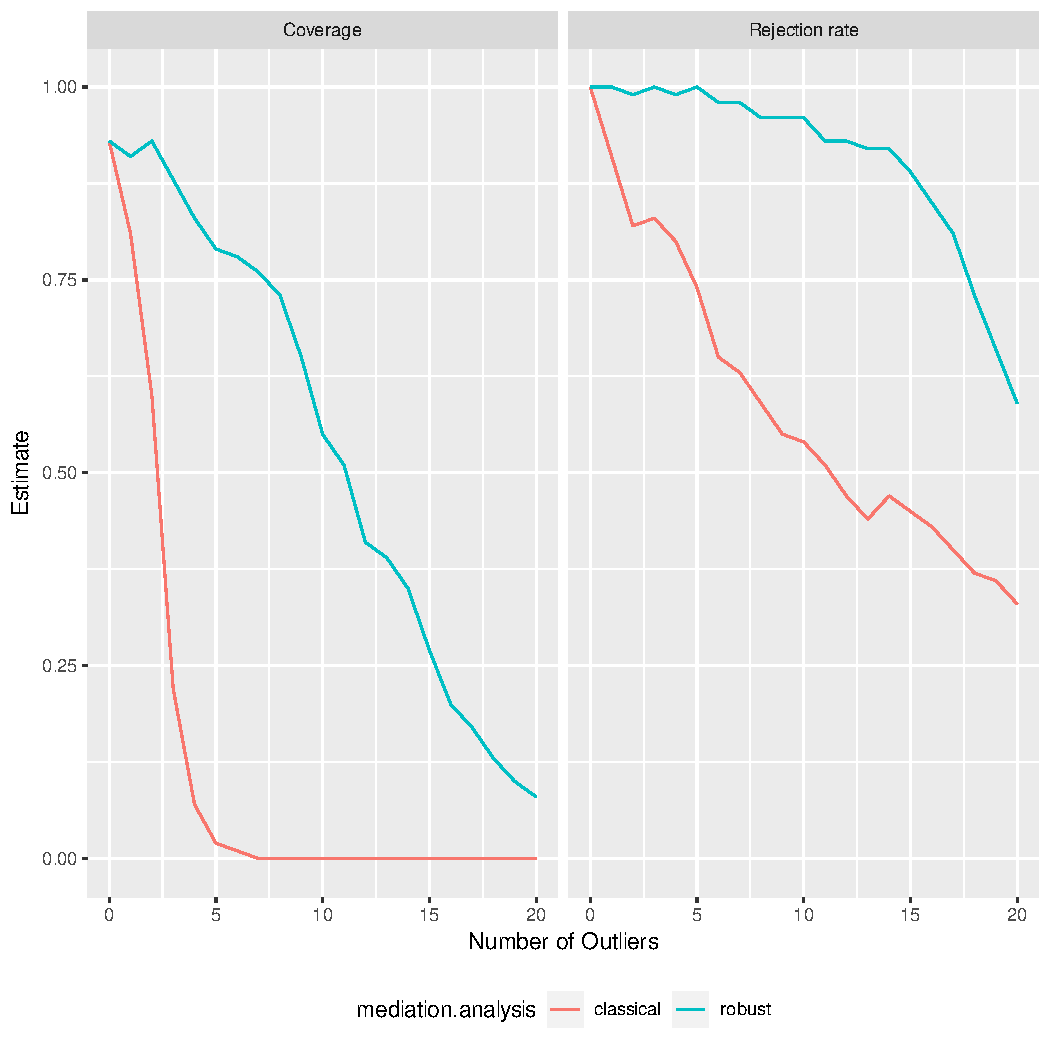
\includegraphics[width = \textwidth]{plot.pdf}
    \caption{Performance of classical and robust mediation analysis on estimating the true indirect effect $\theta_M \beta=1$ in model \eqref{eq:simulation}, with a sample size of $n=100$. The number of outliers is denoted on the $x$-axis. The performance measure ``Coverage'' is the average fraction of times (across the $R=100$ replications) in which the estimated indirect effect is contained in the corresponding boostrapped 95\% confidence interval. The performance measure ``Rejection rate'' is the fraction of times (across the $R=100$ replications) in which the estimated indirect effect is assessed to be statistically significant at the 5\% level (i.e. the value zero is \textit{not} contained in the bootstrapped 95\%  confidence interval).}
    \label{fig:results}
\end{figure}

Figure \ref{eq:simulation} illustrates the rejection rate and coverage of the estimated indirect effect of both the classical and robust mediation analysis across the $R=100$ replications. Already a few outliers are enough to render classical mediation analyses unreliable, as the coverage drops to about 0\% when six out of 100 observations are outliers. Conversely, robust mediation analysis is considerably less affected by outliers and maintains a coverage above 50\% until about ten outliers. Moreover, classical mediation analysis quickly starts to make type II errors in testing the significance of the indirect effect, as the rejection rate drops to below 75\% at already ten outliers. On the other hand, robust mediation analysis is less prone to making type II errors, as its rejection rate only drops below 75\% at about 17 outliers. 

We conclude that robust mediation analysis is indeed more robust against outliers. Therefore, we recommend that researchers working with mediation analysis either carefully screen their datasets for outliers or directly resort to using robust versions of mediation analysis.






\bibliography{paper-bibliography}
\end{document}